\documentclass[12pt,a4paper,twoside,openright]{book}
\usepackage{graphics}
\usepackage{fancyhdr}
\usepackage[latin1]{inputenc}
\usepackage{amsmath,amsfonts,amssymb,amsthm}
\usepackage{epsfig}
\usepackage{deistesi1}
\usepackage{graphicx}
\usepackage{verbatim}
\usepackage{fancyvrb}
\usepackage[italian]{babel}




               %%%%%%%%%%%%%%%%%%%%%%%%%%%%%%%%%%%%%%%%
               % Scelta delle dimensioni della pagina %
               %%%%%%%%%%%%%%%%%%%%%%%%%%%%%%%%%%%%%%%%




               %%%%%%%%%%%%%%%%%%%%%%%%%%%%%%%%%%%%%%
               %  Informazioni generali sulla Tesi  %
               %    da usare nell'intestazione      %
               %%%%%%%%%%%%%%%%%%%%%%%%%%%%%%%%%%%%%%

\frontmatter
\pagestyle{empty}

\titolo{\Huge ALGORITMI DI MACHINE LEARNING PER IL RICONOSCIMENTO VOCALE} \laureando{Elia Favarelli}
\annoaccademico{2016--2017} 
\sessione{II} 
\facolta{Scuola di Ingegneria ed Architettura} 
\corsodilaurea {Ingegneria Elettronica e Telecomunicazioni per l'Energia}
\materia{Elaborazione Numerica dei Segnali LM} 
\relatore[Prof. Ing.]{Andrea Giorgetti} 
\correlatorea[Chiar.mo Prof. Ing.]{Marco Chiani}
\parolechiave{Machine Learning}{Voice Recognition}{Perceptron}{Logistic Regression}{MATLAB}




\pagestyle{fancy}
\renewcommand{\chaptermark}[1]{\markboth{#1}{}}
\renewcommand{\sectionmark}[1]{\markright{\thesection\ #1}}
\fancyhf{} \fancyhead[LE,RO]{\bfseries\thepage}
\fancyhead[LO]{\bfseries\rightmark}
\fancyhead[RE]{\bfseries\leftmark}
\renewcommand{\headrulewidth}{0.5pt}
\renewcommand{\footrulewidth}{0.5pt}


%\addtolength{\voffset}{-5mm} \addtolength{\headsep}{5mm}
%\addtolength{\oddsidemargin}{8mm}
%\addtolength{\evensidemargin}{-8mm}
%\renewcommand{\topmargin}{0pt}
%\addtolength{\headheight}{3pt} \addtolength{\textheight}{10mm}
%\addtolength{\footskip}{10mm}
%
%\linespread{1.25}


\begin{document}

\frontmatter

\maketitle

\tableofcontents

\mainmatter

\chapter*{Introduzione}
\addcontentsline{toc}{chapter}{Introduzione}

L'obiettivo di questo elaborato \`{e} quello di implementare diversi algoritmi che sfruttino alcune fra le pi\`{u} innovative tecniche di classificazione mediante l'approccio del \emph{Machine Learning}. \\

Per \emph{Machine Learning} si intende una particolare classe di algoritmi in grado di \textquotedblleft apprendere\textquotedblright da un set di dati di \emph{training} e successivamente di effettuare delle predizioni su un nuovo set di dati \cite{Machine Learning}. In questa categoria ricadono un gran numero di algoritmi fra cui anche il \emph{Perceptron} e la \emph{Logistic Regression} che verranno ampiamente discussi nel corso dei capitoli successivi.\\

Nella prima parte dell'elaborato verranno indagate le caratteristiche e la struttura di questo tipo di algoritmi, ponendo particolare attenzione ai meccanismi di \emph{learning} che consentono, sotto alcune condizioni, di effettuare una buona classificazione delle misure successivamente sottoposte all'algoritmo.\\

Si proceder\`{a} dunque con un confronto fra i 2 algoritmi sopraccitati, tenendo conto di alcune \emph{features} di interesse quali il tempo di elaborazione e l'accuratezza della classificazione, che pu\`{o} essere stimata con strumenti classici della \emph{teoria della stima} come ad esempio la \emph{matrice di confusione}.\\

Per concludere si caler\`{a} il tutto in un problema reale ovvero la distinzione di 2 voci. L'obiettivo ultimo sar\`{a} dunque quello di riconoscere e distinguere in tempo reale 2 interlocutori che parlano fra loro, a valle di una preventiva fase di \emph{learning} in cui gli interlocutori comunicano separatamente e dichiaratamente.

\clearemptydoublepage

\pagestyle{fancy}
\chapter{Algoritmi di Machine Learning}

Gli \emph{Algoritmi di Machine Learning} trovano interessanti applicazioni in svariati campi e consentono di realizzare classificatori (di cui parleremo in questo elaborato) ma anche stimatori, riconoscitori di pattern e predittori.\\
Il fattore comune a tutti gli algoritmi di \emph{learning} \`{e} proprio la fase di apprendimento.\\ 
Durante questa fase l'algoritmo conosce la classe di appartenenza di una misura, o il pattern che deve riconoscere, o il parametro che deve stimare e setta alcuni parametri al fine di minimizzare l'errore commesso durante la stima.\\
Al termine di questa fase l'algoritmo non conosce pi\`{u} il parametro a priori e cerca di stimarlo al meglio sulla base dell'esperienza acquisita durante la fase di training.\\

\section{Algoritmi di Classificazione}
Concentriamoci quindi sul sottogruppo di \emph{algoritmi di machine learning} utilizzati per effettuare la classificazione, il cui obiettivo \`{e} quello di assegnare una realizzazione alla classe ad essa pi\`{u} affine e pi\`{u} in particolare di algoritmi di classificazione \emph{lineari}, in cui le separazioni fra le varie classi sono di tipo lineare (figura \ref{Fig:Tassonomia degli algoritmi di Machine Learning}).\\
Gli algoritmi di classificazione lineare sono molteplici e si \`{e} deciso di concentrare l'analisi su due di essi in particolare:

\begin{itemize}
	\item Perceptron;
	\item Logistic Regression.
\end{itemize}


\newpage

\begin{figure}[h]
	\centering
	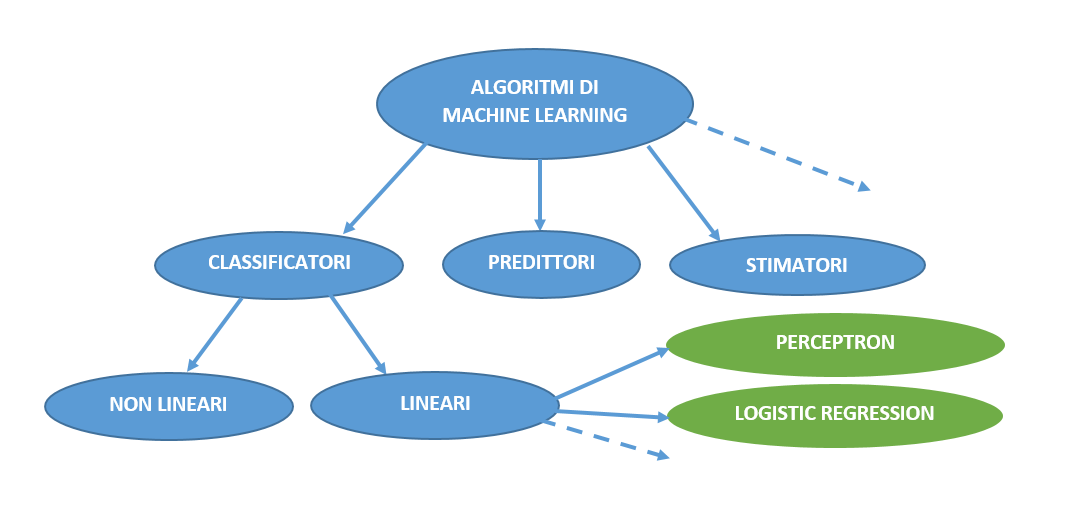
\includegraphics[width=1\textwidth]{Immagini/Classificazione}
	\caption{Tassonomia degli algoritmi di Machine Learning
		\label{Fig:Tassonomia degli algoritmi di Machine Learning}}
\end{figure}


Definiamo di seguito alcuni parametri, vettori e matrici che saranno utili durante la trattazione degli algoritmi:

\begin{description}
	\item[x:] Vettore contenente le \emph{features} estratte dalla misura effettuata (ad esempio energia, ritardo, fase, ampiezza massima, ecc.). Il vettore risulter\`{a} essere m-dimensionale, con una dimensione per ogni \emph{feature} e costituir\`{a} un punto di training (o analogamente una realizzazione);
	\item[X:] Matrice contenente tutti i punti di training, sar\`{a} di dimensioni $N\times M$ con $N$ numero di punti di training; 
	\item[t:] Vettore target contenente le associazioni fra i punti di training e la classe di appartenenza, fornito all'algoritmo durante la fase di learning. Il vettore conterr\`{a} tanti elementi quante sono le misure utilizzate per la fase di \emph{learning} (m-dimensionale);
	\item[]p\textbf{:} Elemento contenente la classe di appartenenza predetta;
	\item[w:] Vettore contenente i pesi calcolati dall'algoritmo in modo da minimizzare l'errore di classificazione, anch'esso di dimensione $N$;
\end{description}

Definiamo inoltre la funzione discriminante utilizzata per la classificazione al termine della fase di learning, che assume la seguente scrittura: 
\begin{equation}
y = \mathbf{w}^T \mathbf{x} + \mathbf{w}_0
\end{equation}
con $\mathbf{w}_0$ termine che tiene conto dell'offset dei punti di learning e $\mathbf{w}^T$ vettore dei pesi \textbf{w} trasposto. Il termine $\mathbf{w}_0$ pu\`{o} essere omesso se si effettua una regolazione dell'offset del problema.


\newpage
\section{Classificazione Multiclasse}
\`{E} doveroso sottolineare come nel caso di classificazione a $K$ classi (con $K>2$) la trattazione si complichi e spesso non sia possibile utilizzare algoritmi che risultavano applicabili nel caso di classificazione a 2 classi (\`{e} il caso ad esempio del \emph{Perceptron}).\\
In letteratura \cite{Bishop} sono riportati vari approcci per estendere il caso di trattazione binaria al caso di $K$ classi, di seguito ne vediamo riportati alcuni, di cui solo 1 risulta per\`{o} essere efficace.

\subsection{One-versus-the-rest classifier} 
Questo approccio prevede di scomporre il classificatore a $K$ classi in $K-1$ classificatori a 2 classi e per ogni classe, verificare se la realizzazione \textbf{x} in ingresso \`{e} pi\`{u} affine alla classe k-esima o a tutte le altre (ecco perch\`{e} il nome \emph{one-versus-the-rest}). Purtroppo agendo in questo modo alcune regioni dello spazio delle realizzazioni rimangono non classificate, ci\`{o} significa che se una realizzazione dovesse cadere all'interno di tale regione non si potrebbe assegnare a nessuna classe (figura \ref{Fig:One-verus-the-rest problem}).

\begin{figure}[h]
	
	\centering
	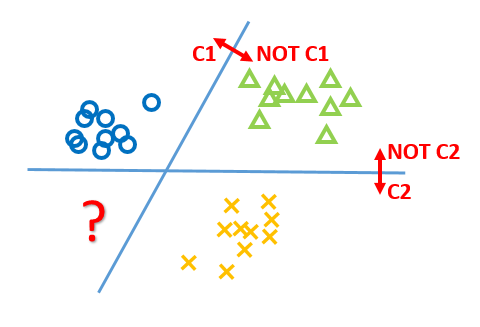
\includegraphics[width=0.9\textwidth]{Immagini/OVTR}
	\caption{One-verus-the-rest problem
		\label{Fig:One-verus-the-rest problem}}
\end{figure}

\subsection{One-versus-one classifier}
In questo caso si considerano invece tutte le possibili coppie di classi e si realizza un classificatore a 2 classi per ciascuna coppia di esse. Agendo in questo modo per\`{o}, oltre ad avere un numero molto elevato di classificatori a 2 classi nel caso di $K$ elevato (le possibili coppie di $K$ classi sono $K(K-1)/2$), si ha anche il problema della sovrapposizione di pi\`{u} classi in alcune regioni dello spazio delle realizzazioni, in tali aree non sar\`{a} dunque possibile risalire alla classe di appartenenza della realizzazione (figura \ref{Fig:One-versus-one problem}).

\begin{figure}[h]
	\centering
	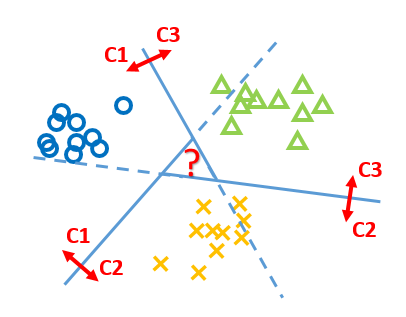
\includegraphics[width=0.8\textwidth]{Immagini/OVO}
	\caption{One-versus-one problem
		\label{Fig:One-versus-one problem}}
\end{figure}

\subsection{Multi-discriminant function}
L'approccio che consente di eliminare ambiguit\`{a} o regioni di spazio non classificate \`{e} quello di utilizzare una funzione discriminante per ciascuna classe ($y_k$), dopodich\'{e} si cerca la classe $k$ che massimizza $y_k$ cos\`{\i} facendo si trova la classe pi\`{u} affine alla realizzazione \textbf{x} ovvero si assegna in maniera esclusiva ogni punto dello spazio ad una classe. Le separazioni delle varie classi saranno quei punti nello spazio delle realizzazioni ove $y_k$ ha valori uguali per almeno 2 valori di $k$ (confine fra 2 classi).


%\input{Capitolo2.tex}
%\input{Capitolo3.tex}
%\input{Capitolo4.tex}
%\input{Capitolo5.tex}
%\input{Capitolo6.tex}
%\input{Capitolo7.tex}


\chapter{Conclusioni}
Con un'accuratezza del 95\% si pu\`{o} affermare che il riconoscitore funziona discretamente, al fine di valutare pi\`{u} a fondo le prestazioni di questa applicazione si potrebbero effettuare in futuro pi\`{u} test variando il tempo di osservazione e il numero di training point per valutare come la distribuzione reale delle realizzazioni infici sull'accuratezza del classificatore.\\

Per aumentare l'accuratezza si pu\`{o} inoltre agire sulla funzione errore, definendo il problema di minimizzazione non pi\`{u} su una funzione di tipo \emph{sigmoide} ma su di una funzione ricavata \textquotedblleft ad hoc\textquotedblright nel caso di distribuzione ad esempio alla \emph{Rayleigh} (la \emph{Logistic Regression} pu\`{o} essere utilizzata per una qualunque funzione appartenente alla classe delle esponenziali di cui la \emph{Rayleigh} fa parte) \cite{Article1}.\\

Per esplorare ulteriormente lo spazio degli algoritmi di machine learning si pu\`{o} inoltre estendere lo studio al caso di pi\`{u} classi, ricercando soluzioni ottime nel caso di 3 o pi\`{u} utenti, oppure sempre nel caso di 2 classi esplorare la categoria di algoritmi non lineari per trovare la soluzione ottima per ogni tipo di distribuzione.

\backmatter

\listoffigures
\addcontentsline{toc}{chapter}{Elenco Figure}

\begin{thebibliography}{20}
\addcontentsline{toc}{chapter}{Bibliografia}

\bibitem{Machine Learning} Andrew Ng: Video Course [Online] 
\begin{verbatim}
https://www.coursera.org/learn/machine-learning/lecture/
Ujm7v/what-is-machine-learning
\end{verbatim}

\bibitem{Bishop} Christopher M. Bishop:  \emph{Pattern Recognition and Machine Learning, Springer-Verlag Ed.},(2006) 

\bibitem{Article1} K.Sithamparanathan and A. Giorgetti, \emph{Cognitive Radio Techniques: Spectrum Sensing, Interference Mitigation and Localization}, Boston, USA: Artech House Publisher, 2012.

\end{thebibliography}
%\input{Ringraziamenti.tex}

\pagestyle{empty}
\cleardoublepage

\end{document}
